
\section{Hybrid Music Recommender}

The hybrid music recommender approach is an implementation of feature augmentation and meta-level methods. One advantage of the meta-level method is the use of compressed users and songs information instead of sparse raw data.
%\begin{itemize}
%\item We model bananas and plums using a density estimation of the colour space.
%\item We fit a Gaussian Mixture Model using Expectation Maximization. We select the number of clusters using an MDL criteria.
%\item Typical image examples of bananas and plums look like this:
%\end{itemize}

\begin{center}
	\resizebox*{0.9\columnwidth}{!}{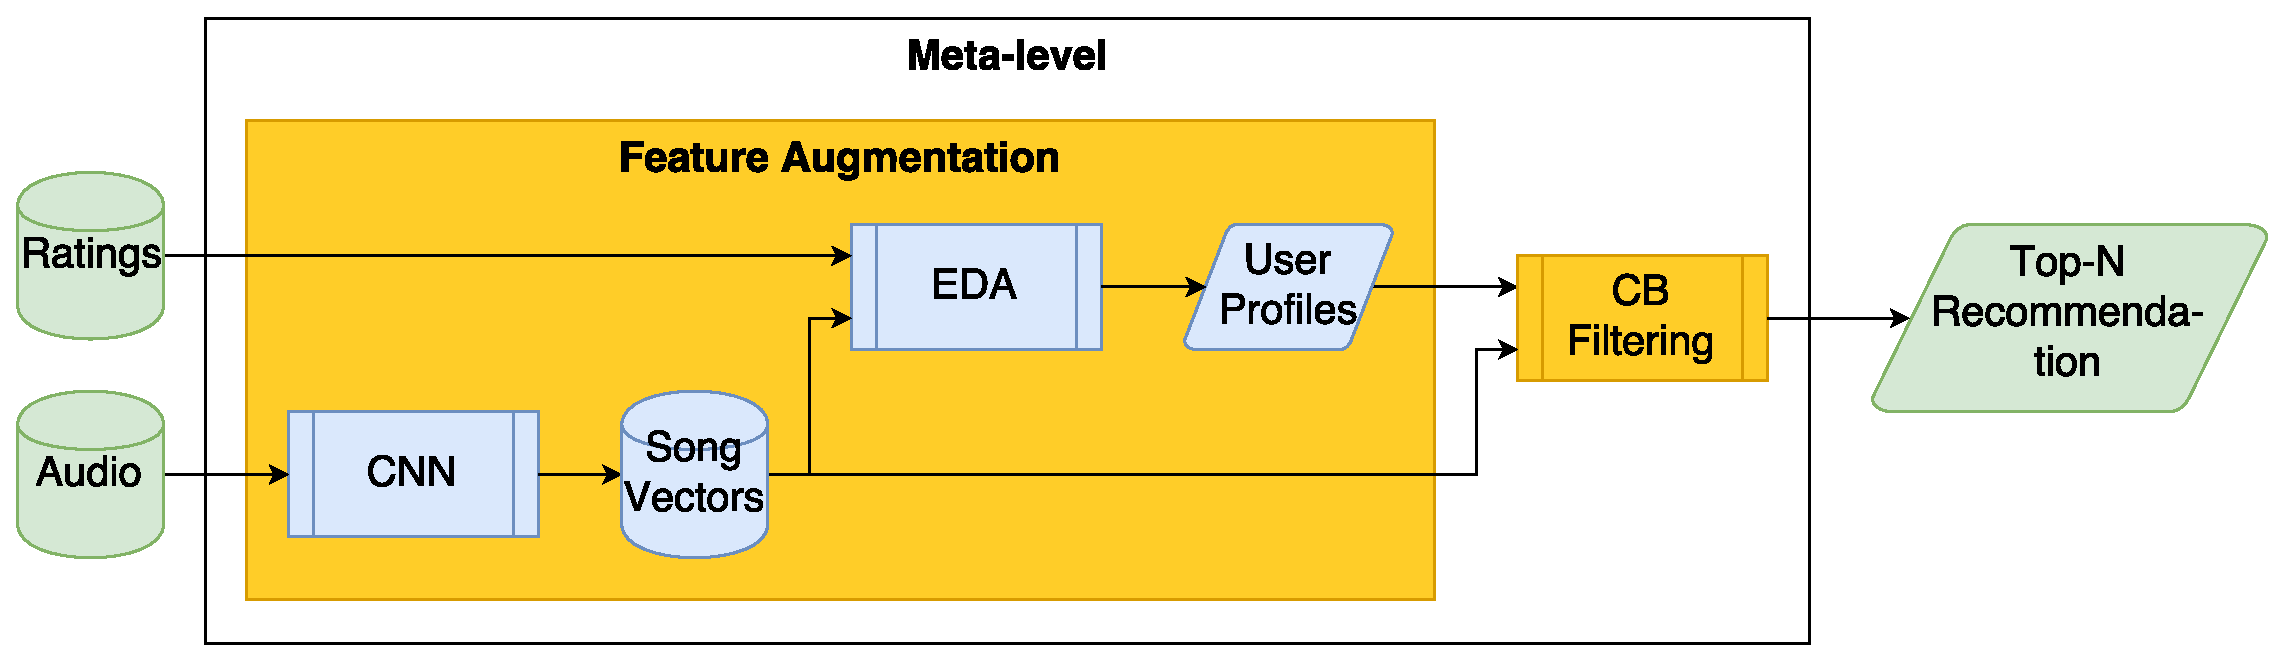
\includegraphics{images/diagram_hybrid_music_recommender.eps}}\\
	{\large \textbf{Fig. 1.} Diagram of our hybrid music recommender approach}
%\begin{tabular}{c@{ }c}
%\resizebox*{0.45\columnwidth}{!}{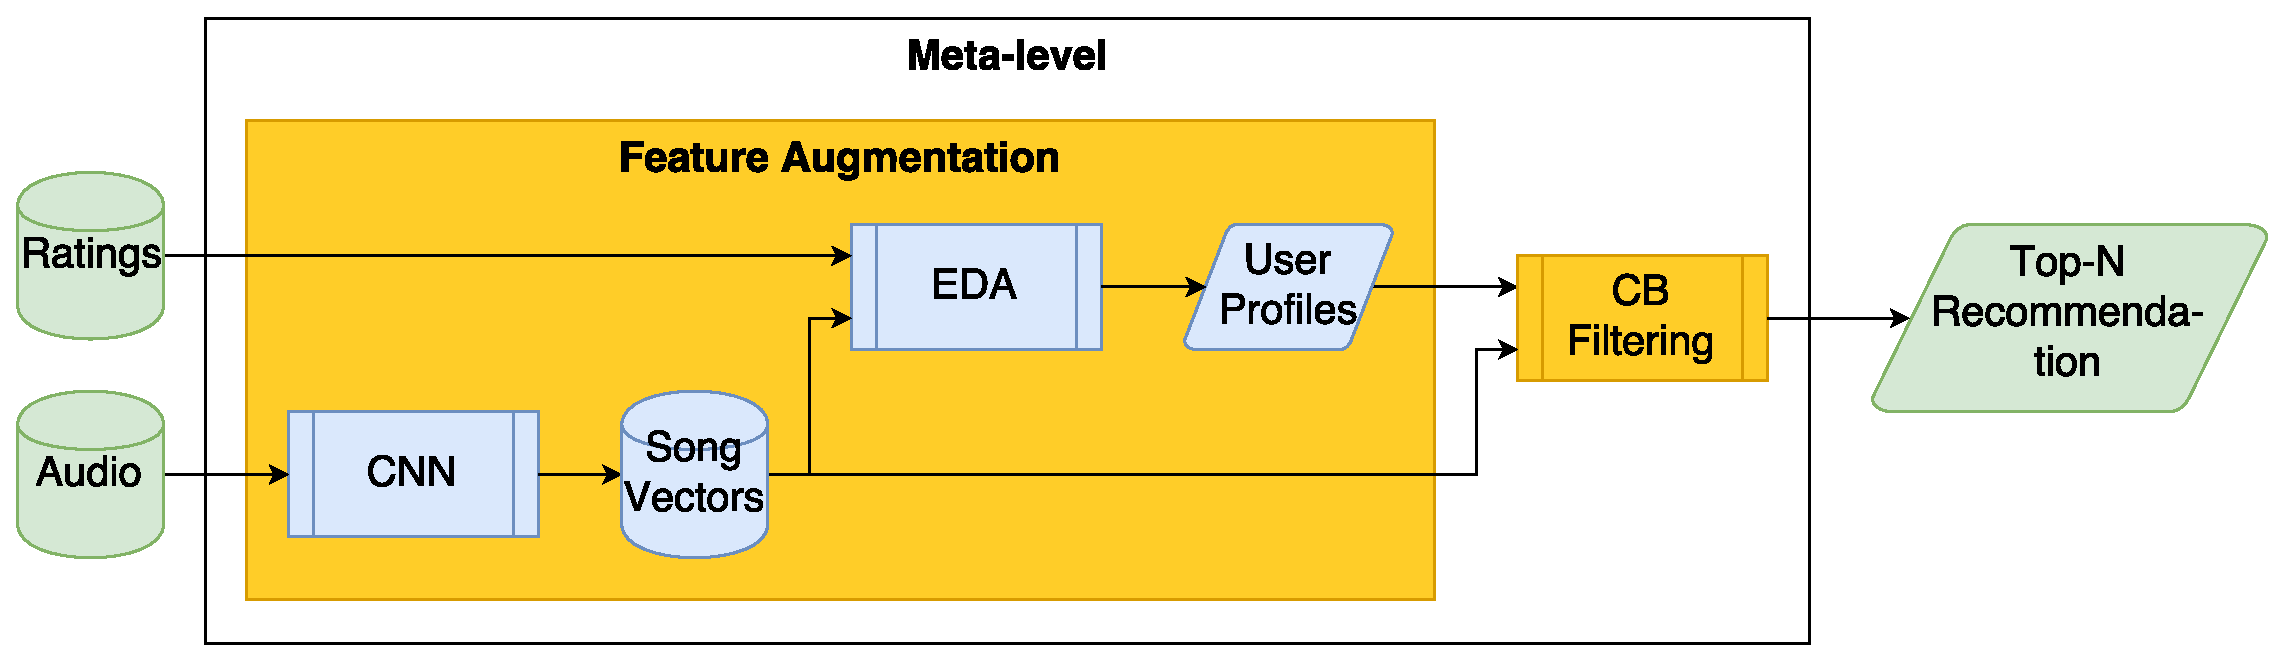
\includegraphics{images/diagram_hybrid_music_recommender.eps}} &
%\resizebox*{0.45\columnwidth}{!}{\includegraphics{images/fruit/plums.eps}} \\
%Bananas & Plums \\
%\end{tabular}
\end{center}
